What do we need this chapter to do?

We need it to set up the background of why something like 3LA needs to exist.
We need it to explain 3LA.
We need it to explain why 3LA needs something like Glenside.


%% Pasted from "overview" 
The past decade has seen the rise
  of specialized hardware
  for
  machine learning accelerators,
  leading to the rise of a
  ``golden age of computer architecture''
  \hl{cite lattner}.
\hl{Statistics on machine learning accelerators}
\hl{Benefits of machine learning
  accelerators; what have they
  enabled.}

Accelerators are difficult to design;
  despite being special-purpose,
  they are nevertheless complex.

A core part of designing an accelerator
  which is often overlooked
  is the process of designing its compiler.
Hardware is nothing
  without software to run on it,
  and your software is only as good as the compiler
  that produces it.
In fact, it isn't uncommon
  for hardware designers in academia
  to simply not design compilers
  for their hardware.

Why is it hard?
Lots has to be written by hand.
Easy to make bugs.
Easy to miss optimizations.

\hl{Existing frameworks for compilers (BYOC) are lacking.}

\hl{Can we make compiler design easier}


\hl{
In part 1 of this disseration,
  I describe an application
  of my thesis
  in the machine learning accelerator space.
I demonstrate how
  formal models of hardware---%
  in this case, captured as rewrites
  over a domain-specific language,
  can be used to automatically generate
  one portion of a compiler.
% Doesn't actually generate it...
% just leans on existing tools!
% but that's kinda what generation is, always...
}


\chapter{Introduction and Motivation}
\label{sec:part1-motivation}

% Top-level points: 
% We need something like the 3LA methodology;
% 3LA methodology needs flexible matching.


% WE NEED SOMETHING LIKE 3LA METHODOLOGY
% Points:
%% Hardware acceleration is important.
%% Accelerators are nothing without testing/without compilers? which one?
%% Need a methodology for building compilers.

%% Hardware acceleration is important.

Hardware acceleration has powered significant advances
  in subfields like artificial intelligence, image processing, and graph analysis~\cite{han2016eie,chen2016eyeriss,reagen2016minerva,zhang2016cambricon,hameed2010understanding,ham2016graphicionado}.
\hl{glenside} Machine learning (ML) and other
  high-performance computing (HPC)
  applications increasingly rely on
  specialized hardware accelerators to
  provide speed and energy efficiency~\cite{jouppi2017tpu, krizhevsky2012conv, reuther2019survey}.
This trend has highlighted the need
  for flexible accelerator support
  in domain-specific compilers like
  Halide~\cite{halide},
  TVM~\cite{tvm},
  TensorFlow/MLIR~\cite{tensorflow, mlir}, and
  PyTorch~\cite{pytorch}.



%% Accelerators are nothing without testing/without compilers? which one?

Core to developing
  accelerators
  quickly and correctly
  is the process of \textit{hardware validation.}
\hl{glossary terms: validation, testing, verification}
\textit{Validation}
  of hardware---%
  the process of testing
  whether the hardware behaves
  how the designer intended---%
  is important.
An immense amount of effort
  and money
  is currently put
  into hardware validation and testing.
\hl{how much is spent on hw validation compared to sw}  

\begin{figure}[!ht]
  %\centering
  \begin{minipage}[h]{0.49\textwidth}
    \vspace{-5\fboxsep}
    \caption{
    \hl{this figure is taken from ...cite 3LA...update caption}
    \textbf{Gap in end-to-end evaluation of accelerators for neural network applications:} 
    Survey of papers from ISCA, MICRO, VLSI, and ISSCC in 2021 and ICCAD, DAC in 2020.
    Our survey of $79$ papers  that introduced new DL accelerator designs/methodologies, comparing how the accelerators were evaluated. Only 41\% of the works reported end-to-end evaluation on non-synthetic applications, of which 68\% (28\% of the total) were from industrial teams.
    }
    \label{fig:3la-pie}
  \end{minipage}\hfill
  \begin{minipage}[h]{0.49\textwidth}
    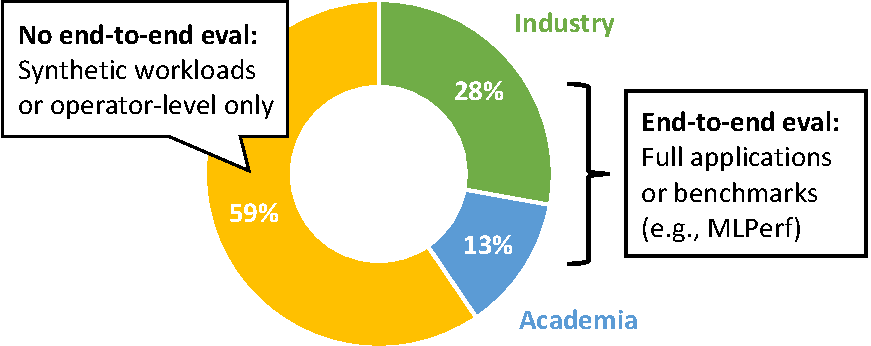
\includegraphics[width=\textwidth]{assets/3la-pie.pdf}
  \end{minipage}
\end{figure}


In general,
  thorough validation
  is inaccessible
  to the common designer.
The most intensive validation
  is done in industry,
  where companies can hire full-time
  engineers
  to do validation
  on designs.
\hl{reference fig} \cref{fig:3la-pie}
  
When validation \textit{is} done
  outside of industry,
  it is often not done end-to-end.
Not only is it important
  to test \textit{components}
  of a hardware design;
  it is also important
  to test full applications end-to-end.
Hardware specialization and customization often
  requires changing memory hierarchies,
  data representations~\cite{chan2014itrs,fang2019understanding,lai2021programming}.
Issues arising from these complex
  microarchitectural changes
  may not manifest
  at the component level---%
  for example, a reduced-bitwidth
  ALU
  may still produce accurate results,
  but overal \textit{application}
  performance
  may suffer
  due to the change in numeric behaviors.
\hl{call forward to evaluation}
Testing is often 
  too commonly poorly done.
\hl{insert figure from 3LA}

%% Need a methodology for building compilers.

In response to the challenges
  of hardware validation
  to the common designer,
  the authors of \hl{cite 3LA}
  developed
  a methodology
  to make testing
  easier for new accelerator designs.
The primary contribution of 3LA
  is 
  a methodology to end-to-end evaluate accelerators on unmodified, full applications.
Explain how we're just a component of 3LA.

\begin{figure}
    \centering
    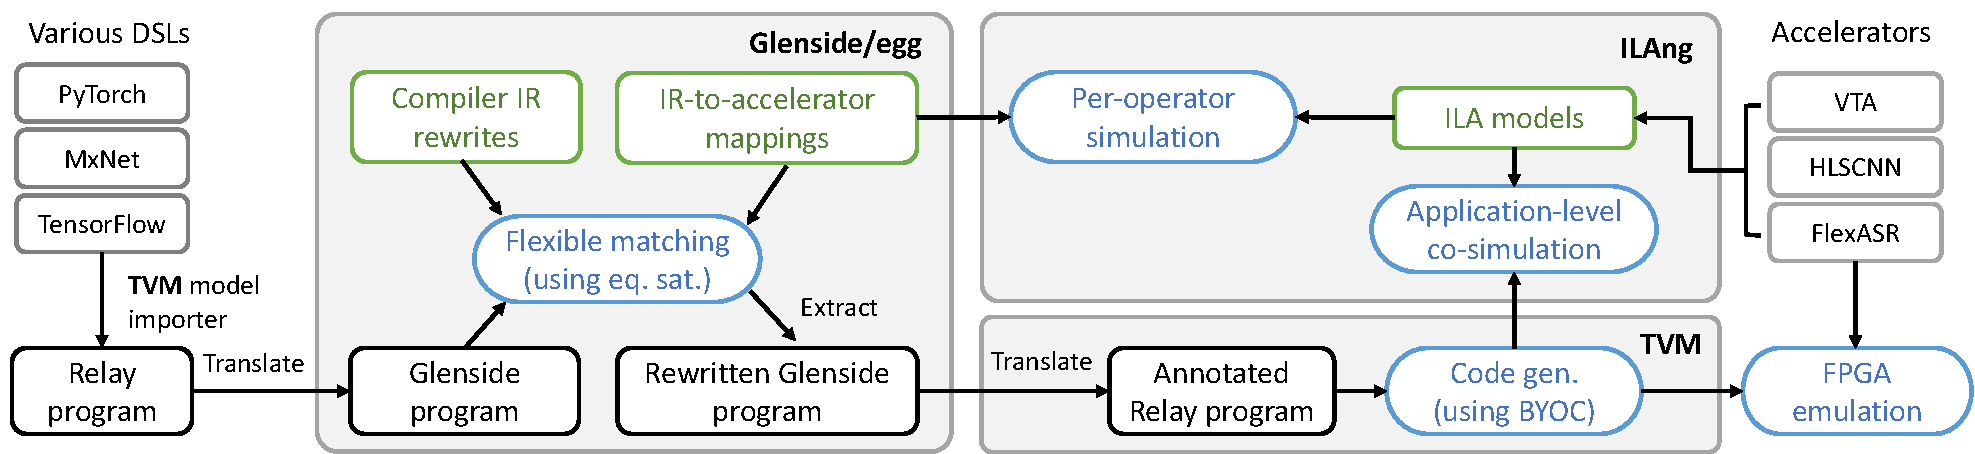
\includegraphics[width=\textwidth]{assets/3la-diagram.pdf}
    \caption{
    \hl{not quite sure where this goes}
This figure first appeared
  in Huang et.~al.~\cite{3la}.
Diagram of the 3LA prototype's flow.
Note that only the ``Glenside/egg''
  portion of 3LA
  is considered a contribution
  of this dissertation;
  for more information on the other components,
  please see the original paper.
}
    \label{fig:3la-diagram}
\end{figure}

3LA solves two major problems:
  first, generating simulators
  for hardware
  is difficult
  and time consuming.
Second, even given a simulator
  for your design,
  it is then difficult
  to run full applications
  on the simulator.
The first contribution
  of 3LA
  we do not consider
  a contribution of this thesis;
  please refer to the dissertation
  of Bo-yuan Huang
  \hl{ref his thesis.}

However,
  the second contribution of 3LA
  results directly from contributions
  of this thesis.
One of the challenges
  that 3LA solves:
  compiling to custom hardware is hard.
This is where I was able
  apply my dissertation.
We developed a language
  called \g
  which allowed for the application
  of equality saturation


%% GLENSIDE INTRO

Adding accelerator support to
  an existing compiler typically
  uses custom pattern matching to
  map expensive tensor operations
  from applications down to
  accelerator invocations~\cite{
    yang2020interstellar, byoc}.
Pattern matching often additionally relies on
  various other transformations
  to canonicalize intermediate representations (IRs)
  %~\cite{??}
  and massage data layouts into
  formats matching accelerator requirements~\cite{nvidia2020nhwc}.
Even with these changes,
  users may need to manually modify their application to
  help the compiler discover opportunities
  for dispatching operations to accelerators, 
  such as by changing data types or unrolling loops.
\hl{
These modifications may be especially
  untenable
  for hardware developers,
  who may not have practical experience
  with the workloads
  and toolchains. 
(something tying it in to new combined intro)
}
    
In principle, term rewriting techniques~\cite{baader1998term}
  should be able to facilitate many of
  these transformation and mapping tasks
  within a compiler.
Halide and TVM already rely
  on extensive rewrite systems for
  optimizing scalar computations and
  simplifying loop bounds in order to
  support further downstream optimizations~\cite{newcomb2020halide-rewrite,
  hagedorn2020func-high-perf}.

Unfortunately, existing IRs in compilers for
  array/tensor programming DSLs tend to
  present abstraction and granularity mismatches
  that hamper term rewriting approaches.
Term rewriting is most easily applied in
  \textit{pure} (side effect--free) IRs
  that support equational reasoning.
At the same time,
  mapping to accelerators requires considering
  low-level hardware details like data layout.
Existing pure IRs for ML frameworks are used
  primarily for high-level transformations
  (e.g., type elaboration and inlining)
  and do not expose low-level data layout details~\cite{relay}.
On the other hand,
  IRs used for crucial lower-level optimizations like
  operator fusion must support
  precise reasoning about memory use,
  and therefore are typically impure,
  hampering term rewriting.% approaches.

To help mitigate such impedance mismatches,
  we present \textit{\g},\footnote{Publicly available at \url{https://github.com/gussmith23/glenside}.}
  a pure tensor program IR
  that enables hardware-level term rewriting.
\g is based on a simple
  \textit{access pattern} abstraction that
  supports expressing and reasoning about
  data layout transformations via
  syntactic rewrite rules.
  \begin{wrapfigure}{r}{.5\textwidth}
    \centering
    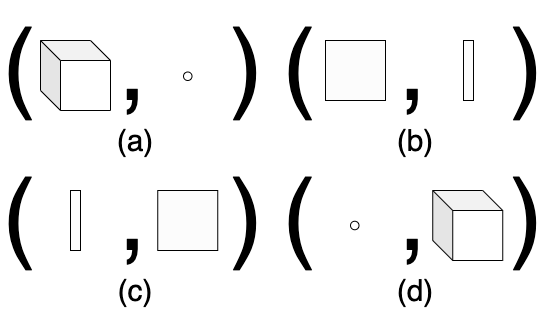
\includegraphics[width=.9\linewidth]{glenside/access-pattern-examples-2x2.png}
    \caption{
      Four access patterns,
        representing different ways
        a
        tensor program
        (or \textit{kernel})
        might access
        the same 3D tensor. 
      For example, (c) represents
        accessing a 3D tensor as
        a vector of 2D matrices.}
    \label{fig:access-pattern-examples}
    \vspace{-1em}
\end{wrapfigure}
When combined with standard arithmetic rewrites
  for per-tensor-element computations,
  access patterns enable implementing complex
  transformations for accelerator support as
  compositions of simple rewrites.

Tensors are traditionally characterized
  by their \textit{shape},
  an $n$-tuple 
  %in $\mathbb{N}^n$
  of positive integers
  indicating the size of each
  of a tensor's dimensions.
  % , e.g., $(x, y, z)$ for a 3D tensor.
Access patterns instead characterize
  each tensor with two shapes, e.g.,
  \accesspatternshape{x}{y, z}, separating
  the dimensions which are \textit{iterated over} from
  the dimensions which are \textit{computed on.}
Figure~\ref{fig:access-pattern-examples}(c)
  depicts an example where a 3D tensor's
  first dimension is iterated over and
  some computation applied to each
  corresponding 2D matrix.

\g \hl{
 plays a crucial role in the 3LA framework.
}
We demonstrate how \g
  enables implementing representative
  hardware-level transformation via term rewriting,
  including mapping computations
  to systolic arrays~\cite{jouppi2017tpu}
  (a common hardware module in ML accelerators)
  and automatically discovering the
  \tcd{im2col} data layout transformation~\cite{im2col},
  which enables mapping 2D convolutions
  to matrix multiplication hardware.
In particular,
  by employing \textit{equality saturation}~\cite{willsey2021egg},
  these transformations ``fall out for free''
  (i.e., without any carefully crafted
  rewrite orderings~\cite{phase-ordering}),
  from a handful of general rewrites concerning tensor
  transposition, Cartesian product, dot product, etc.,
  expressed in terms of access patterns.


\hl{move this to glenside chapter?}
 The rest of this chapter is organized as follows:
Section~\ref{sec:background} provides background
  and briefly surveys closely related work.
Section~\ref{sec:matmul} motivates
  \g via a running example exploring
  pure matrix multiplication.
Section~\ref{sec:glenside} details the
  design and implementation of \g.

%% END GLENSIDE INTRO

Skipping over the comparisons with related work.
If we include anything, it should be something
  from the Task 1 paraagraph, re comparison with Exo, MLIR, etc.

Should take something from "detailed comparison
  with closely related tools".

Background. Can probably skip 2.1.

Probably want 2.2. But maybe should just be the Glenside chapter.

But then we need to find a way
  to lead into the Glenside intro.

Would be great to set up this chapter
  so that it ends with a very clear statement
  of what we need our language to do.
Then the Glenside chapter can do those things.
But we also need to make sure
  we tie it back to the thesis.


  To summarize, the contributions of this chapter include:
\begin{itemize}
\item \textit{Access patterns},
  a tensor representation that employs a
  simple, extended tensor shape type to
  distinguish iteration and computation dimensions

\item The \g IR,
  a pure compiler IR that facilitates 
  term rewriting to enable support for
  specialized accelerators
  
\item A library of generic rewrites over \g programs
  
% \item Case studies demonstrating how
%   \g enables automatically discovering
%   key transformations for mapping
%   applications to custom accelerators
%   via equality saturation with the
%   \tcd{egg}~\cite{willsey2021egg} library.
\end{itemize}


% 3LA methodology needs flexible matching.
\section{3LA Methodology}


We now give a description
  of the structure
  of the 3LA methodology